\chapter{Test plan}\label{ch:test}

For the verification of the correctness of our implementation of
\cordic{} is to write a \matlab{} model of the algorithm and then compare the
output to the VHDL one.

To run the tests described below, do the following:
\begin{enumerate}
	\item Open \code{matlab/Cordic.prj} in \matlab;
	\item Run \code{cordic\_float} to execute the floating point model
		described in \secref{sec:float};
	\item Run \code{cordic\_quantized} to execute the quantized model
		described in \secref{sec:quantized} and generate input files for
		the \modelsim{} testbench;
	\item Open \code{CORDIC/Modelsim/CORDIC.mpf} in \modelsim;
	\item Compile and run the simulation (testbench file:
		\code{cordic\_tb.vhd});
	\item Get back to \matlab{} and run \code{VHDL\_output\_verification},
		then you can check the various computed values and errors in the
		\matlab{} workspace.
\end{enumerate}

Note that, in the following, only the most important \matlab{} scripts are
shown. The full \matlab{} scripts set is available as attachment to this
document.

\section{Floating Point Model}\label{sec:float}

The first model we have to write is a floating point version of \cordic{}
algorithm as we can see in \lstref{lst:cordicfloatmatlab}.

\lstinputlisting[language=matlab, label={lst:cordicfloatmatlab},
caption={CORDIC Floating Point Model in Matlab
(\code{cordic\_vectoring\_float.m}).}]{matlab/float/cordic_vectoring_float.m}

From this model we can obtain a measure of the algorithmic error, comparing the
output of this algorithm, produced with a test input dataset\footnote{The test
input dataset is composed by points lying on circumferences with different
radius}, and compared to the radius and phase computed in ``traditional'' way.

The result is that both on phase and radius the error after 14 iterations is in
the order of \(10^{-9\) for the radius (as shown in
\figref{fig:floaterrorradius}) and \(10^{-4}\) for the phase (as shown in
\figref{fig:floaterrorphase}). The resulting \emph{Mean Square Errors} and
\emph{Max Errors} are shown in~\eqref{eq:errorfloat}.

\begin{equation}\label{eq:errorfloat}
	\begin{array}{rl}
		MSE_r &= 2.8876\times10^{-18}\\
		MSE_p &= 4.2575\times10^{-9}\\
		MaxError_r &= 6.3350\times10^{-9}\\
		MaxError_p &= 1.1865\times10^{-4}
	\end{array}
\end{equation}

\begin{figure}[htb]
	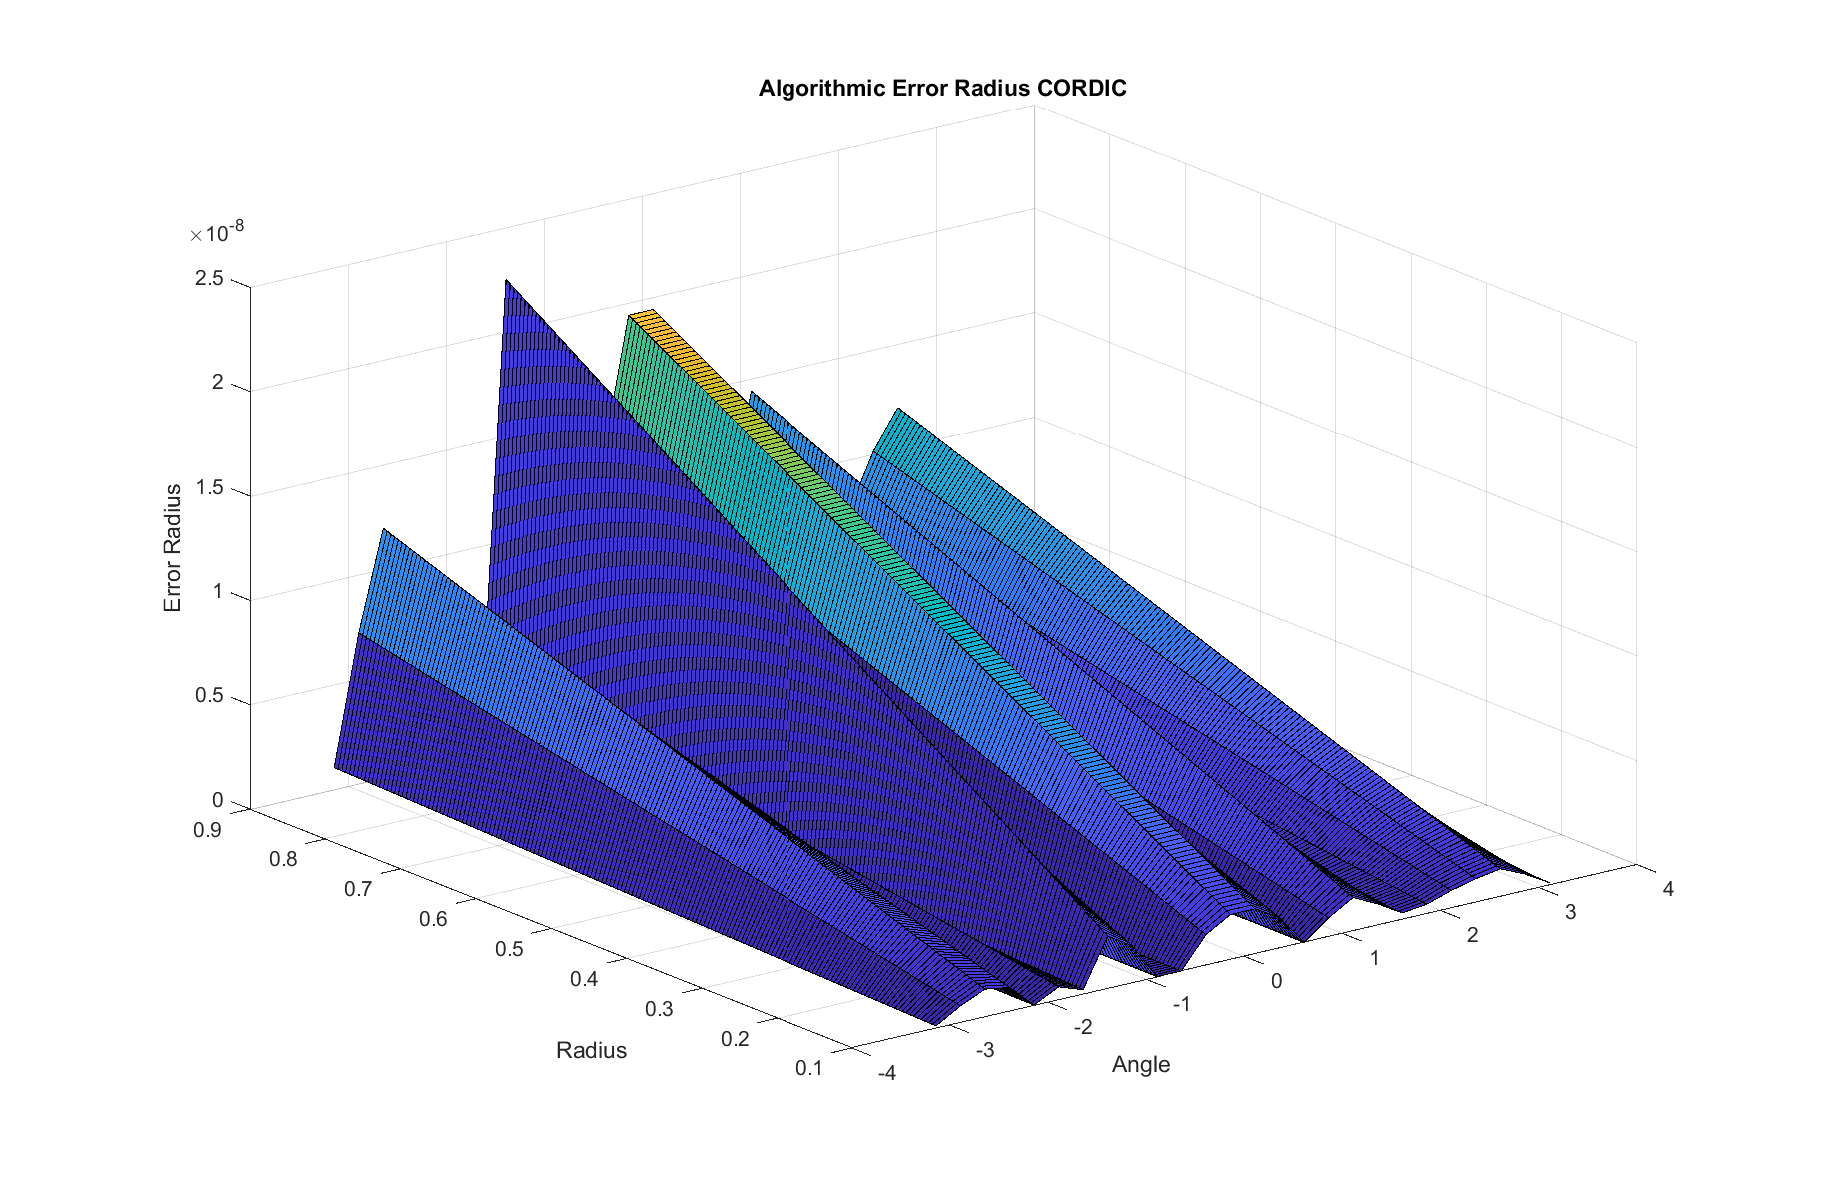
\includegraphics[width=\textwidth]{alg_error_radius}
	\caption{Algorithmic Error Radius.}\label{fig:floaterrorradius}
\end{figure}
\begin{figure}[htb]
	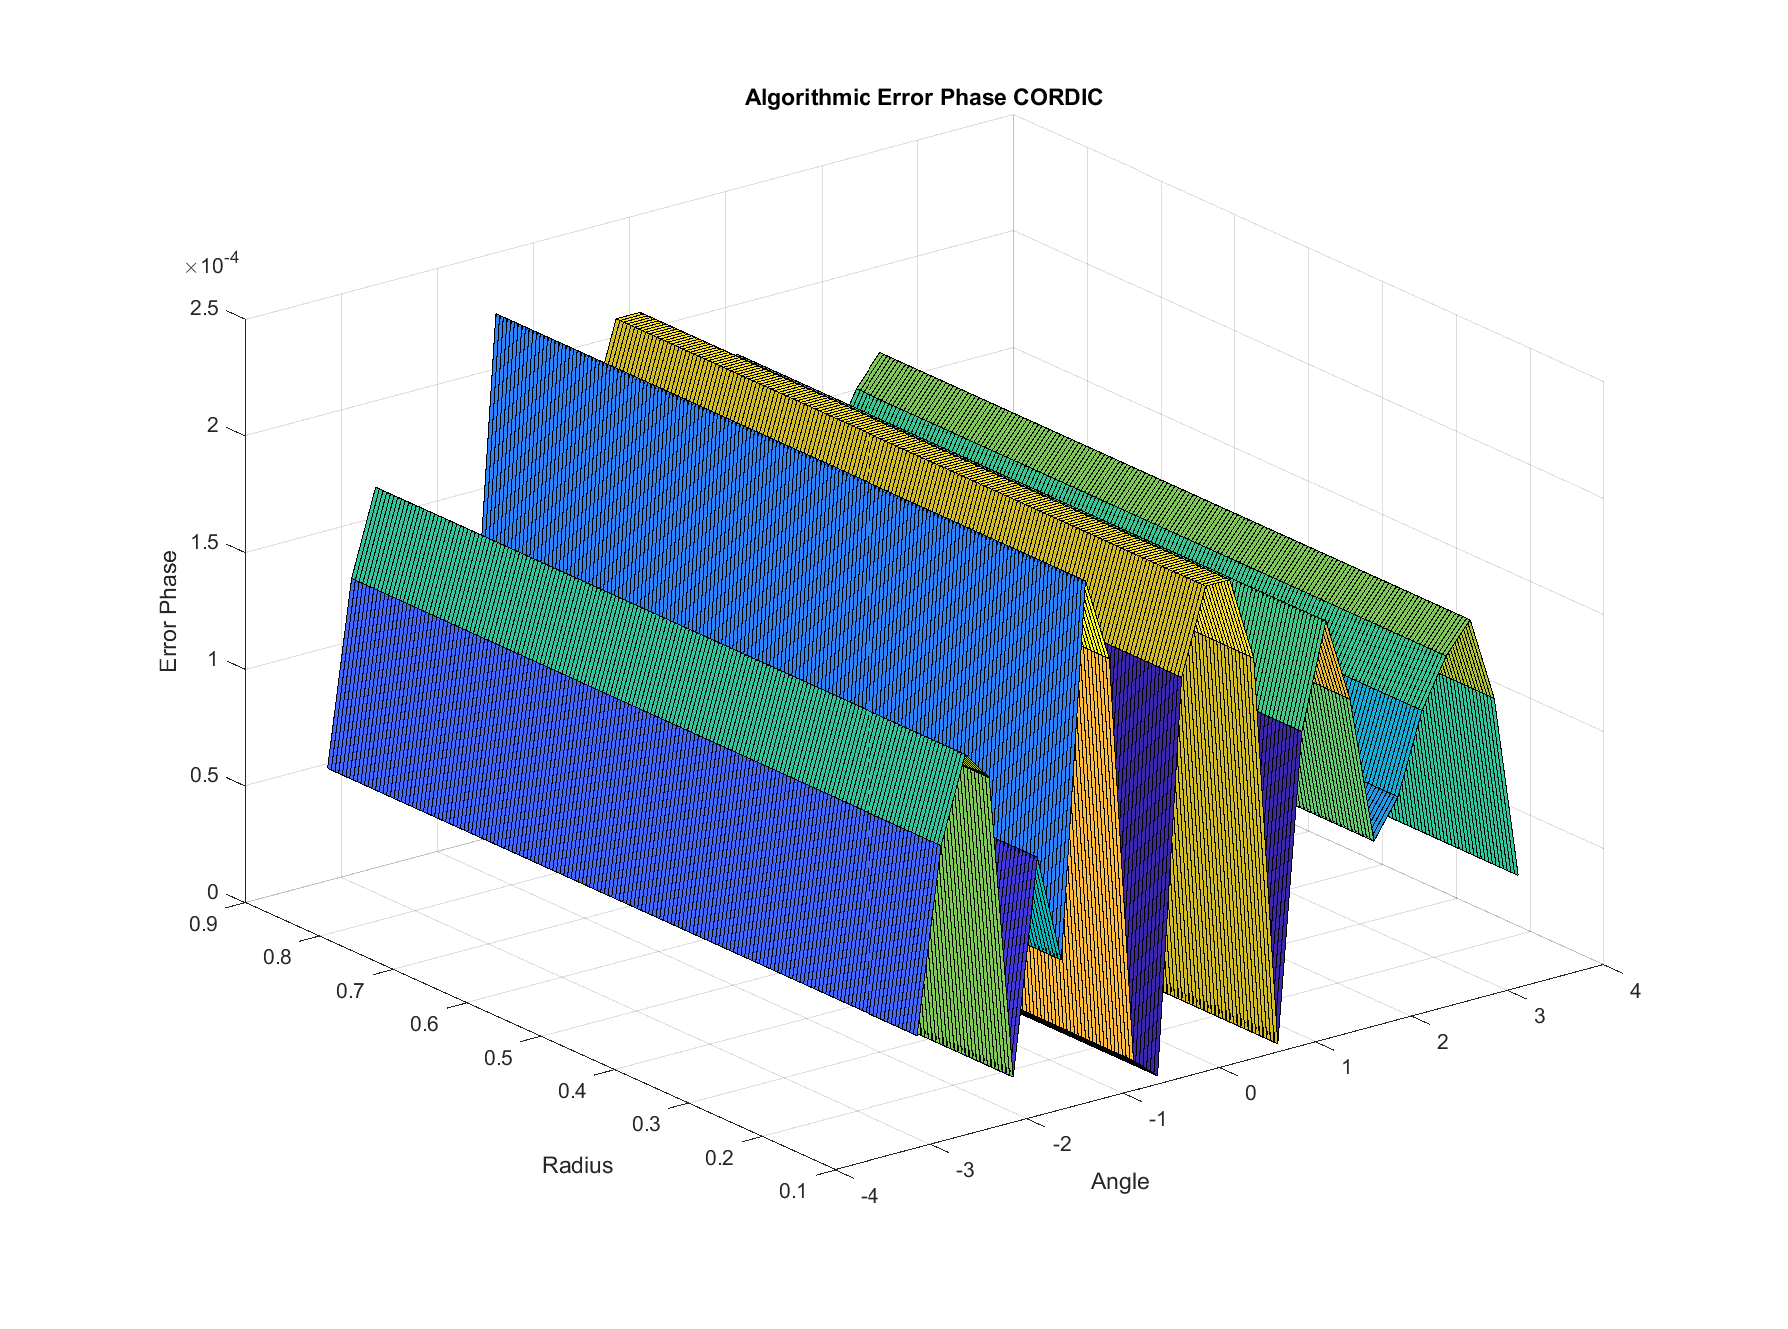
\includegraphics[width=\textwidth]{alg_error_phase}
	\caption{Algorithmic Error Phase.}\label{fig:floaterrorphase}
\end{figure}

\section{Quantized model}\label{sec:quantized}

After the floating point model we moved towards lower level, performing a
quantization of input values.

To do that we have to fix their dimensions in bits, that will be the same of the
VHDL implementation, after that we have to fix the range of acceptable \(x\),
\(y\) and \(phase\) values so that we can compute the \emph{LSB} value for
\(x\), \(y\) and \(phase\) as shown in \lstref{lst:cordicq}.

\lstinputlisting[language=matlab, label={lst:cordicq},
caption={CORDIC Quantized Model in Matlab
(\code{cordic\_quantized.m}).}]{matlab/quantized/cordic_quantized.m}

The output of this model with the same inputs given to the floating point model
gives us the opportunity to evaluate the quantization error introduced. In
\figref{fig:qerrorradius} we can appreciate the quantization error on the radius
and in \figref{fig:qerrorphase} the quantization error on the phase.


\begin{figure}[htb]
	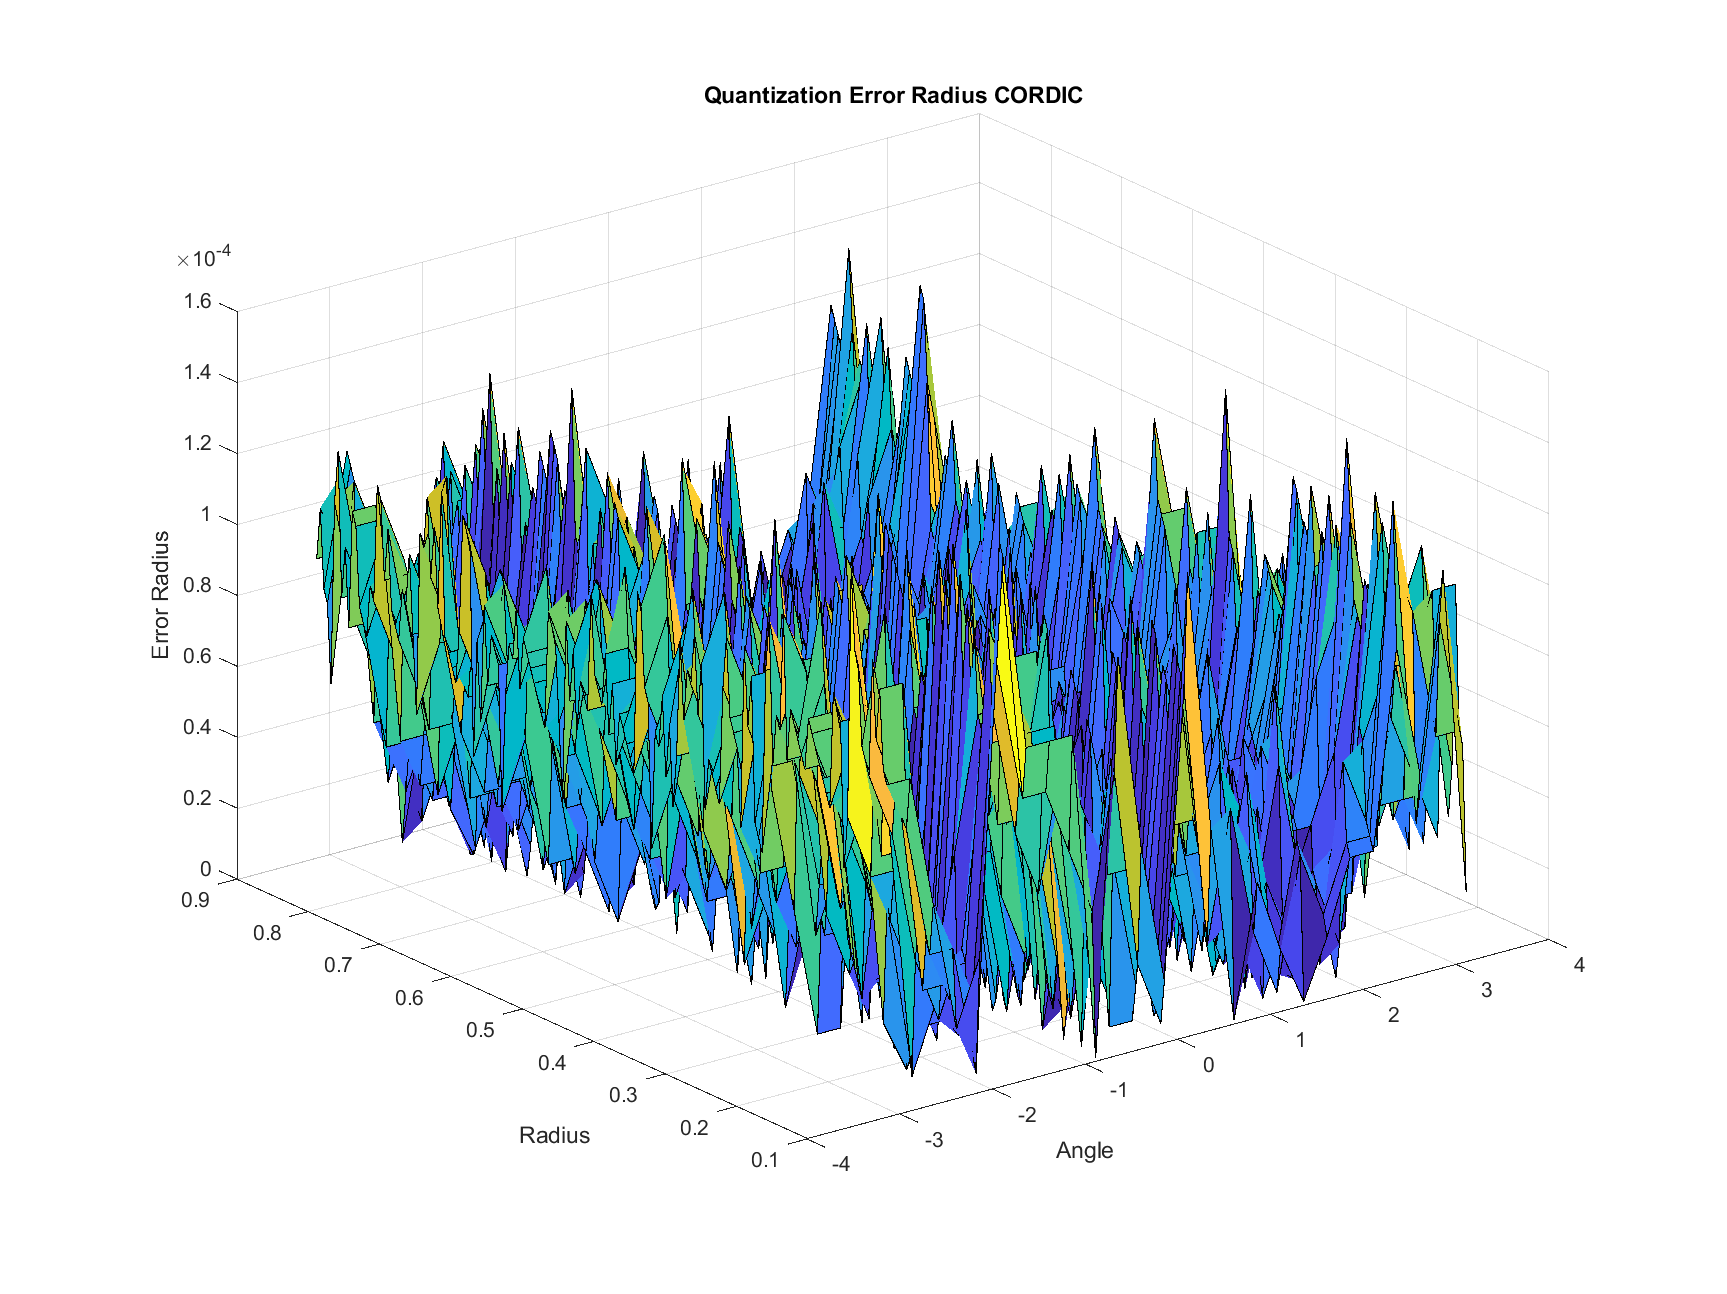
\includegraphics[width=\textwidth]{quant_error_radius}
	\caption{Quantization error Radius}\label{fig:qerrorradius}
\end{figure}
\begin{figure}[htb]
	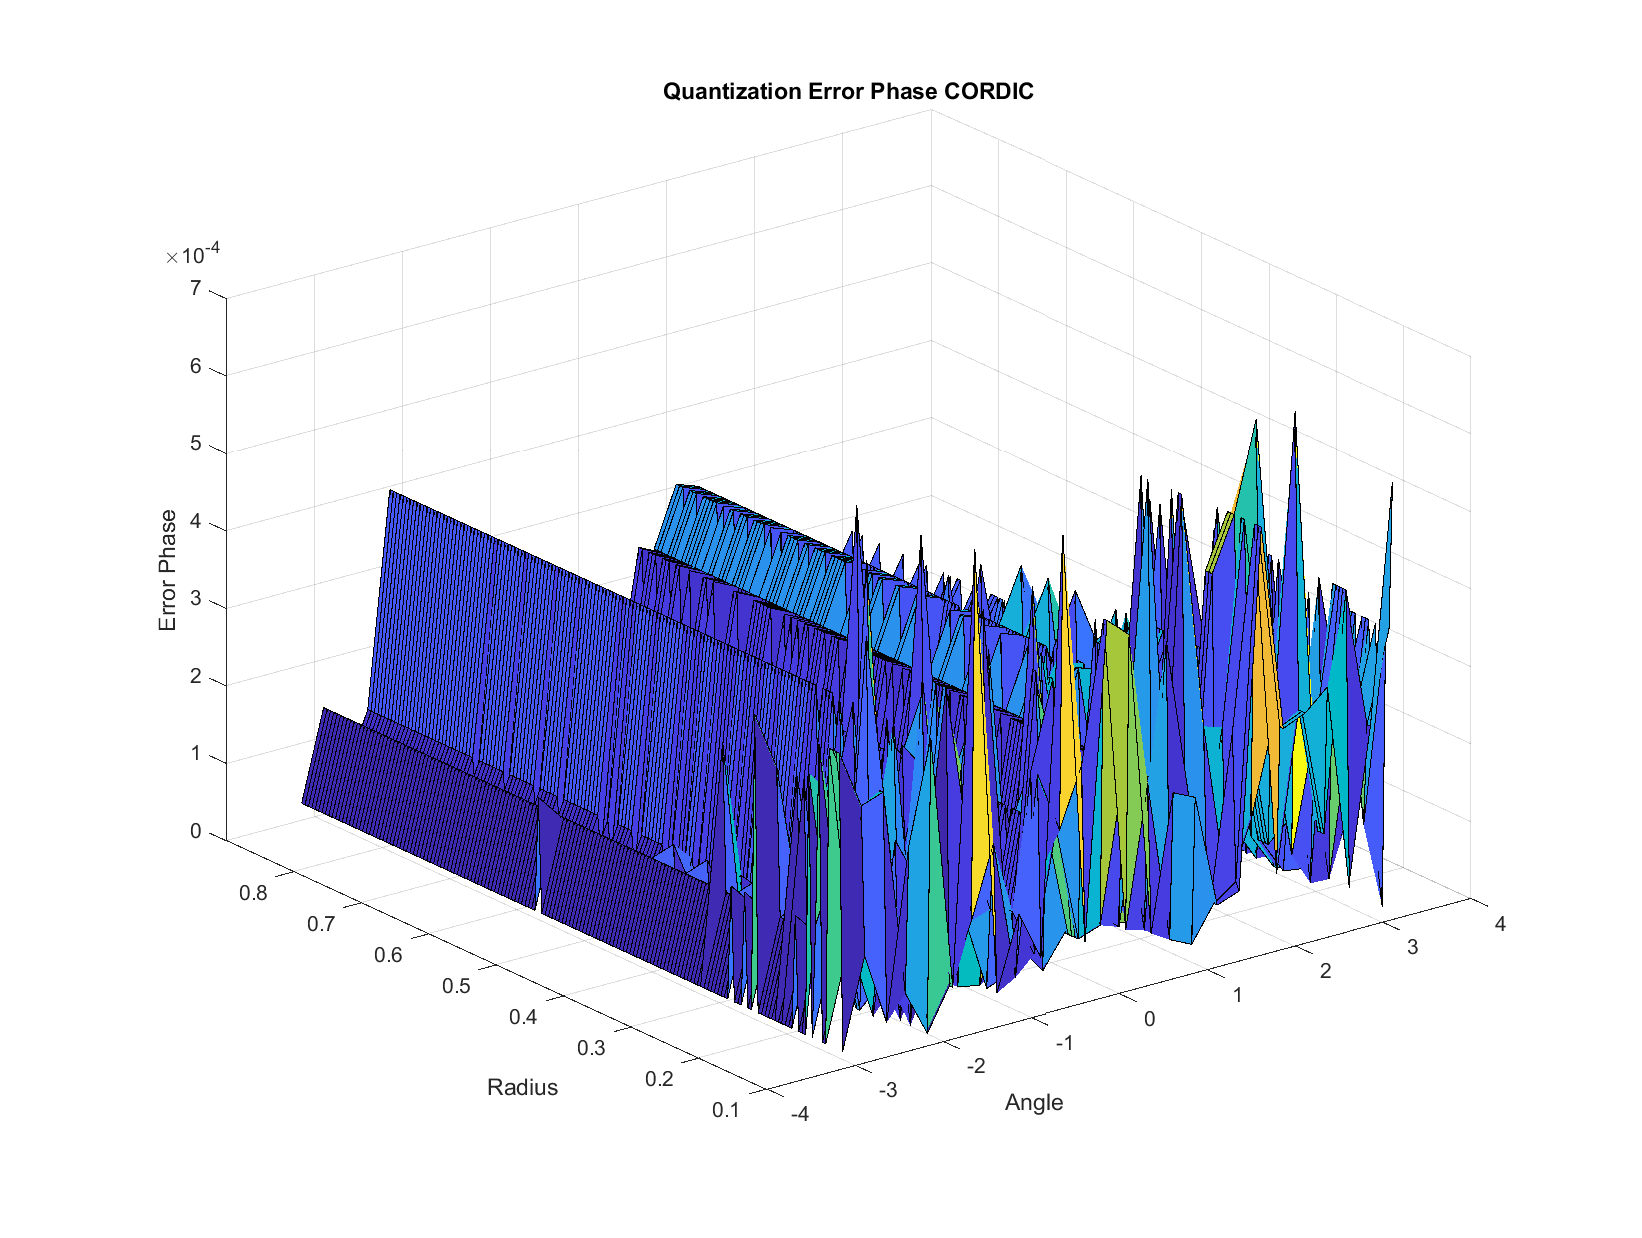
\includegraphics[width=\textwidth]{quant_error_phase}
	\caption{Quantization error Phase}\label{fig:qerrorphase}
\end{figure}

\section{VHDL model test}\label{sec:vhdltest}

The last step is to check te correctness of our implementation. To do that we
have to extract the output from the implementation through a simulation with
the testbench shown in \lstref{lst:testbench}.

\lstinputlisting[language=vhdl, label={lst:testbench},
caption={CORDIC testbench
(\code{cordic\_tb.vhd}).}]{CORDIC/hdl/tb/cordic_tb.vhd}


Then we can compute the error of the \matlab{} model with respect to the
implementation. A correct implementation should have an output completely equal
to the quantized model's one.

The test performed in \lstref{lst:vhdloutputver} confirm that our implementation
is completely compliant with the \matlab{} model, thus is correct.

\lstinputlisting[language=matlab, label={lst:vhdloutputver},
caption={VHDL output verification in Matlab
(\code{VHDL\_output\_verification.m}).}]{matlab/VHDL_output_verification.m}

